\documentclass[10pt, a5paper]{article}
\usepackage{pdfpages}
\usepackage{parallel}
\usepackage[T2A]{fontenc}
\usepackage{ucs}
\usepackage[utf8x]{inputenc}
\usepackage[polish,english,russian]{babel}
\usepackage{hyperref}
\usepackage{rotating}
\usepackage[inner=2cm,top=1.8cm,outer=2cm,bottom=2.3cm,nohead]{geometry}
\usepackage{listings}
\usepackage{graphicx}
\usepackage{wrapfig}
\usepackage{longtable}
\usepackage{indentfirst}
\usepackage{array}
\newcolumntype{P}[1]{>{\raggedright\arraybackslash}p{#1}}
\frenchspacing
\usepackage{fixltx2e} %text sub- and superscripts
\usepackage{icomma} % коскі ў матэматычным рэжыме
\PreloadUnicodePage{4}

\newcommand{\longpage}{\enlargethispage{\baselineskip}}
\newcommand{\shortpage}{\enlargethispage{-\baselineskip}}

\def\switchlang#1{\expandafter\csname switchlang#1\endcsname}
\def\switchlangbe{
\let\saverefname=\refname%
\def\refname{Літаратура}%
\def\figurename{Іл.}%
}
\def\switchlangen{
\let\saverefname=\refname%
\def\refname{References}%
\def\figurename{Fig.}%
}
\def\switchlangru{
\let\saverefname=\refname%
\let\savefigurename=\figurename%
\def\refname{Литература}%
\def\figurename{Рис.}%
}

\hyphenation{admi-ni-stra-tive}
\hyphenation{ex-pe-ri-ence}
\hyphenation{fle-xi-bi-li-ty}
\hyphenation{Py-thon}
\hyphenation{ma-the-ma-ti-cal}
\hyphenation{re-ported}
\hyphenation{imp-le-menta-tions}
\hyphenation{pro-vides}
\hyphenation{en-gi-neering}
\hyphenation{com-pa-ti-bi-li-ty}
\hyphenation{im-pos-sible}
\hyphenation{desk-top}
\hyphenation{elec-tro-nic}
\hyphenation{com-pa-ny}
\hyphenation{de-ve-lop-ment}
\hyphenation{de-ve-loping}
\hyphenation{de-ve-lop}
\hyphenation{da-ta-ba-se}
\hyphenation{plat-forms}
\hyphenation{or-ga-ni-za-tion}
\hyphenation{pro-gramming}
\hyphenation{in-stru-ments}
\hyphenation{Li-nux}
\hyphenation{sour-ce}
\hyphenation{en-vi-ron-ment}
\hyphenation{Te-le-pathy}
\hyphenation{Li-nux-ov-ka}
\hyphenation{Open-BSD}
\hyphenation{Free-BSD}
\hyphenation{men-ti-on-ed}
\hyphenation{app-li-ca-tion}

\def\progref!#1!{\texttt{#1}}
\renewcommand{\arraystretch}{2} %Іначай формулы ў матрыцы зліпаюцца з лініямі
\usepackage{array}

\def\interview #1 (#2), #3, #4, #5\par{

\section[#1, #3, #4]{#1 -- #3, #4}
\def\qname{LVEE}
\def\aname{#1}
\def\q ##1\par{{\noindent \bf \qname: ##1 }\par}
\def\a{{\noindent \bf \aname: } \def\qname{L}\def\aname{#2}}
}

\def\interview* #1 (#2), #3, #4, #5\par{

\section*{#1\\{\small\rm #3, #4. #5}}

\def\qname{LVEE}
\def\aname{#1}
\def\q ##1\par{{\noindent \bf \qname: ##1 }\par}
\def\a{{\noindent \bf \aname: } \def\qname{L}\def\aname{#2}}
}

\switchlang{ru}
\begin{document}
\title{Измеряем океан мензуркой (оценка характеристик глобальной сети)}
% \author{Александра Кононова, Moscow/Zelenograd, Russian Federation, \linebreak Алексей Городилов, Russian Federation} % не лезет!
\author{Александра Кононова, Алексей Городилов, \\ Russian Federation\footnote{\url{illinc@bk.ru}, \url{https://lvee.org/ru/abstracts/317}}}
\maketitle
\begin{abstract}
% Описан эксперимент по оцениванию распределения длин путей между узлами в~глобальной сети и~его характеристик.
% В~частности, показана методика измерения длины пути от узла $\alpha$ к узлу $\beta$ при помощи утилиты GNU/Linux traceroute и~ограничения выбора узлов $\alpha$ и~$\beta$, налагаемые этим инструментом.
% Приведены результаты измерений.
% Описана имитационная модель эксперимента, разработанная для проверки корректности полученных оценок распределения длин путей между узлами в~глобальной сети.
% Показано, что глобальная сеть не описывается моделью Барабаши"--~Альберт, но может быть в~некотором приближении описана разработанной  предфрактальной моделью.
The experiment, aimed at finding the distribution of path lengths between nodes in the global network and estimation of parameters of that distribution is described. 
At particular, described the method of measurement of path length from node $\alpha$ to the node $\beta$ with traceroute utility of the GNU/Linux system, and limitations on the selection of nodes $\alpha$ and $\beta$, imposed by trace\-route.
Measurements results are given and analyzed.
Simulation model of this experiment was developed to test the experiment validity in the determination of distribution parameters in the global network. This model is also described. 
It is shown that the global network could not be described by Barab\'{a}si-Albert model, but it could be described with some approximation by developed and proposed a pre-fractal model.
\end{abstract}

\subsection*{Введение}


Разработка эффективных сетевых приложений невозможна без сведений о структуре сети, в которой они будут работать. Так, в 2011 году, для получения параметров методики МУчОС~\cite{muchos} передачи мультимедийных данных с учётом особенностей сети, был начат эксперимент по оценке распределения длин путей  сетевого уровня модели TCP/IP глобальной сети.

Определим понятие длины пути и~распределения длин путей.
Из-за 
% особенностей 
свойств
стека протоколов TCP/IP, если от узла $\alpha$ к узлу $\beta$ в~принципе возможна передача данных,  маршрут передачи данных на сетевом уровне будет единственным.
Пусть это $\alpha \to \alpha_1 \to \ldots \to \alpha_{k-1} \to \beta$. 

% Тогда количество $k$ пересылок узел-узел в этом маршруте будем называть длиной пути от узла $\alpha$ к узлу $\beta$:
% $$
% s(\alpha, \beta) = k,
% $$

Тогда длина  $s(\alpha, \beta)$ пути от узла $\alpha$ к узлу $\beta$ "--- количество $k$ пересылок узел-узел в этом маршруте.
При этом $s(\alpha_{k-1}, \beta) = 1$, ...  $s(\alpha_1, \beta) = k-1$.

Со временем глобальная сеть изменяет свою структуру, и как маршрут передачи данных, так и~его длина $s(\alpha, \beta)$ могут изменяться.
Кроме того,
из-за особенностей маршрутизации может быть $s(\alpha, \beta) \neq s(\beta, \alpha)$.
% ; кроме того, как $s(\alpha, \beta)$, так и маршрут передачи данных от $\alpha$ к $\beta$ может изменяться во времени. При этом в каждый момент времени $s(\alpha_1, \beta) = s(\alpha, \beta) - 1$ и т. д.

Таким образом, под распределением длин путей графа $G$ 
понимается ряд чисел $\zeta(x)$, показывающий, как часто длина $x$ встречается среди всех возможных путей в~$G$:
$$
\zeta(x) = p \big(
s(\alpha,\beta)=x ~ | ~ \alpha,\beta \in G
\big).
$$
Непосредственно измерить распределение длин путей $\zeta(x)$ для глобальной сети (то есть измерить и~проанализировать длины $s(\alpha, \beta)$ для всех возможных пар $(\alpha, \beta)$) невозможно как из-за её гигантских размеров, так и~из-за отсутствия в~стеке TCP/IP средств для измерения расстояния между двумя произвольно взятыми узлами.


\subsection*{Выбираем мензурку}

Для исследования маршрутов сетевого уровня в~GNU/Linux \linebreak предназначена утилита traceroute.
При запуске в~командной строке узла $\alpha$ команды \mbox{\texttt{traceroute $\beta$}} результатом будет маршрут передачи данных $\alpha \to \alpha_1 \to \ldots \to \alpha_{k-1} \to \beta$, причём одна строка вывода traceroute соответствует одному узлу маршрута.
Далее путём синтаксического анализа можно определить длину пути $s(\alpha, \beta)$.

Таким образом, для измерения длины пути $s(\alpha, \beta)$  необходимо иметь право на запуск программ на узле 
$\alpha$ (в~дальнейшем будем называть его корневым, рис.~\ref{ei_rdp}) и~знать IP-адрес или имя узла  $\beta$ (будем называть его оконечным).
\begin{figure}[h!]
  \centering
  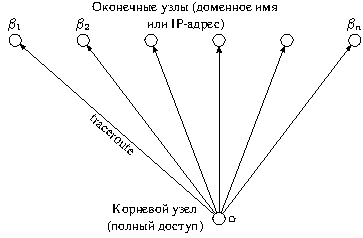
\includegraphics[width=0.7\linewidth]{2019_miet_kai_gav_ei_rdp}
\caption{Схема измерений выборочных длин путей}
\label{ei_rdp}
\end{figure}%
Также необходима возможность соединения $\alpha$ с~$\beta$, то есть оконечный узел $\beta$ должен иметь белый IP-адрес либо находиться в~одной подсети с~$\alpha$.

Ограничения на выбор оконечного узла гораздо мягче, чем для корневого.
Соответственно, количество возможных оконечных узлов может быть намного больше (множество оконечных узлов $Q=\{\beta_1, \beta_2, \ldots \beta_n \}$ на рис.~\ref{ei_rdp}).



Соответственно, задавшись парой из корневого узла $\alpha$ и~множества оконечных узлов $Q$ и~измеряя при помощи traceroute расстояния $s(\alpha, \beta_j)$ от 
$\alpha$ до каждого из оконечных $\beta_j \in Q$, можно получить 
% долю путей 
некоторую оценку распределения длин путей $\zeta(x)$ глобальной сети.
Эта оценка зависит от выбора корневого узла, от множества оконечных узлов и~от времени (от текущей конфигурации глобальной сети).


%Соответственно, граф, вершинами которого являются все доступные узлы глобальной сети (с белыми IP-адресами), а рёбрами "--- ???, является деревом.
В ходе этого эксперимента были сформированы три различных множества оконечных узлов ($P, R, T$ размерами  564, 5222 и~540 уникальных белых IP-адресов соответственно)
и~три корневых узла ($A, H, M$).


Так как все оконечные узлы имели белые IP-адреса, а~корневые "--- серые,
каждый маршрут передачи данных $\alpha \to \alpha_1 \to \ldots \to \alpha_{k-1} \to \beta$
от корневого узла $\alpha$ до оконечного узла $\beta$ делился на две части:
 маршрут от корневого узла $\alpha$ до шлюза $\alpha_{gw}$ его провайдера $\alpha \to \ldots \to \alpha_{gw}$
и~маршрут от шлюза провайдера корневого узла до оконечного узла $\alpha_{gw}\to \ldots\to \alpha_{k-1} \to \beta$.

Для каждой пары корневого узла $\alpha$ и~оконечного узла $\beta$ получались два значения длины пути:
полная длина $\widetilde{s}(\alpha, \beta) = k$, включающая подсеть  провайдера корневого узла
и~скорректированная длина ${s}(\alpha, \beta) = k-gw$, исключающая подсеть  провайдера корневого узла (то есть включающая только пересылки между узлами с~белыми IP-адресами).

После окончания измерений множества полученных значений длин путей $\widetilde{s}$ и~$s$ обрабатывались GNU Octave.
% 
Соответственно, для каждой пары корневого узла $\alpha$ и~множества оконечных узлов $Q$ получались две оценки распределения длин путей:
$\widetilde{\zeta}(x)$, включающая подсеть  провайдера корневого узла
и~$\zeta(x)$, исключающая подсеть  провайдера корневого узла.


\subsection*{Оцениваем}

От корневых узлов $A$ и~$M$ было выполнено по четыре разнесённых во времени измерения расстояний до каждого из наборов $P$, $R$, $T$;
от узла $H$, из-за ограниченного времени доступа "--- только по одному измерению до каждого из наборов $P$, $R$, $T$.
Таким образом, всего было выполнено 27~измерений и~получено 27 оценок $\widetilde{\zeta}(x)$ распределения длин путей, включающих подсеть провайдера корневого узла (рис.~\ref{zplot_2x1}, а)
\begin{figure}[h!]
  \centering
  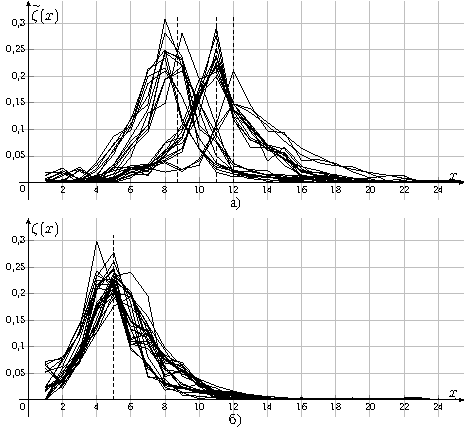
\includegraphics[width=\linewidth]{2019_miet_kai_gav_zplot_2x1}
\caption{Экспериментально полученное распределение длин путей:
а) включая подсеть провайдера корневого узла,
б)~исключая подсеть провайдера корневого узла
}
\label{zplot_2x1}
\end{figure}%
и~27 оценок~$\zeta(x)$ распределения длин путей, исключающих подсеть провайдера корневого узла (рис.~\ref{zplot_2x1}, б).

В~соответствии с~множеством оконечных узлов, корневым узлом и~порядковым номером измерения
обозначены как $PA_0, PA_1, PA_2,$ $PA_3,$ $PH_0, PM_0, \ldots PM_3,$ $RA_0, \ldots RM_3, TA_0, \ldots TM_3$
и~перечислены на рис.~\ref{5x2_experiment_moments} именно в~таком порядке.

\begin{figure}[p]
  \centering
  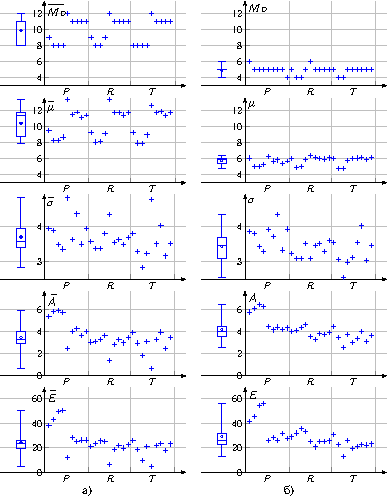
\includegraphics[width=\linewidth]{2019_miet_kai_gav_5x2_experiment_moments}
\caption{Характеристики экспериментально полученных оценок распределения длин путей:
а) включая подсеть провайдера корневого узла,
б)~исключая подсеть провайдера корневого узла
}
\label{5x2_experiment_moments}
\end{figure}

Рис.~\ref{5x2_experiment_moments}, а) показывает разброс характеристик (моды $Mo$, среднего $\mu$, среднеквадратического отклонения $\sigma$, асимметрии $A$ и~эксцесса $E$) оценок $\widetilde{\zeta}(x)$ распределения длин путей, включающих подсеть провайдера корневого узла.
% По оси абсцисс 
Ось абсцисс соответствует номеру измерения, как сказано выше; 
% измерения сгруппированы по множеству оконечных узлов ($P$, $R$, $T$ "--- границы групп показаны линиями сетки), затем по корневому узлу
% % , внутри каждой группы упорядочены по 
% и~времени ($A_0$, $A_1$, $A_2$, $A_3$, далее $H_0$ и~$M_0$, $M_1$, $M_2$, $M_3$).
границы между измерениями, соответствующими множествам оконечных узлов $P$, $R$, $T$  показаны линиями сетки.
% 
Слева от оси ординат разброс показан в~виде ящика с~усами (усы соответствуют минимальному и~максимальному значениям, края ящика "--- первой и~третьей квартилям, линия внутри ящика "--- медиане, кружок "--- среднему значению характеристики).
 
Рис.~\ref{5x2_experiment_moments}, б) аналогично показывает разброс характеристик оценок $\zeta(x)$ распределения длин путей, исключающих подсеть провайдера корневого узла.

Значение эксцесса $E$ здесь и~далее вычисляется по формуле с~коррекцией на три (так, чтобы эксцесс нормального распределения был бы равен нулю).

Видно, что значения асимметрии и~эксцесса оценок распределения длин путей (как $\widetilde{\zeta}(x)$, так и~$\zeta(x)$) существенно больше нуля.

\subsection*{Поверяем}

Насколько корректны полученные оценки $\zeta(x)$?
% 
Для их проверки было сгенерировано некоторое количество графов $G$, размеры которых позволяют:
\begin{itemize}
	\item[--]рассчитать расстояние $s(\alpha, \beta)$ для всех возможных пар узлов $\alpha, \beta \in G$ и~рассчитать истинное (полное) распределение длин путей $\zeta(x)$;
	
	\item[--] %а~также 
	выполнить имитацию эксперимента и~оценить  $\zeta(x)$ по 
заданным корневому узлу $r$ и~множеству оконечных узлов $Q$.
\end{itemize}
Размеры множеств $Q$, использованных в~экспериментальном исследовании, составляют $500-5000$ узлов.
Соответственно, минимальным количеством вершин в~$G$ в~расчётах было $|G| = 10^3$ узлов.
Максимальным размером $G$, при котором можно выполнить расчёт менее чем за месяц "--- $|G| = 10^6$ узлов.

Граф $G$ из~$|G|$ вершин представлялся в~памяти компьютера в~виде сжатой матрицы смежности,
то есть вектором $\rho_G$ из~$|G|$ списков,
каждый из которых соответствует вершине графа  и~содержит номера смежных с~ней вершин.
% Таким образом, элемент вектора $\rho_G$ с~номером $i \in [0, |G|)$ соответствует вершине $\nu_i$ и~хранит список вершин, смежных с~$\nu_i$.

% Как для расчёта 
Для расчёта длин путей использован  поиск в~ширину,
позволяющего для заданной вершины  $\alpha \in G$ рассчитать расстояния до всех прочих вершин графа $G$.
Таким образом, результат соответствует экспериментальным измерениям для корневой вершины $\alpha$ и~множества оконечных вершин $Q=G$, включающего все вершины графа.
Сложность поиска в~ширину для представления графа в~виде $\rho_G$  равна $O(|G| +|E_G|)$, где $|E_G|$ "--- количество рёбер~\cite{Sedgewick2002_AlgorithmsinC_Fundamentals}.
Таким образом, при расчёте полного распределения длин путей все вершины $\alpha \in G$ графа  поочерёдно рассматриваются в~качестве корневых, и~сложность возрастает в~$|G|$ раз.
Для ускорения расчёта  использован компилируемый язык C++ (стандарт C++11) и~распараллеливание OpenMP.

Кроме полного распределения длин путей $\zeta(x)$, для каждого графа $G$ рассчитывались ещё 
% Для каждого дерева $G$ рассчитывалось как полное распределение длин путей $\zeta(x)$, так  и~
несколько оценок $\zeta(x)$ по разным парам  $(r,Q)$ корневой узел-множество оконечных узлов. 
Эти оценки обозначались $\zeta_i(x)$.
%  , где $i$ "--- порядковый номер .

Корневая вершина $r$, как и~оконечные вершины $\beta_j \in Q$ для каждого $i$ выбиралась случайно.
Количество оконечных вершин $|Q|$ во время предварительных вычислений варьировалось в~диапазоне $500-5000$ узлов.
Так как не было выявлено существенного различия результатов, для итогового моделирования было принято $|Q|=500$.

Таким образом, аналогом выполненных в~эксперименте измерений (оценивания распределения длин путей глобальной сети по нескольким корневым узлам и~нескольким выборкам оконечных узлов)
является один прогон модели, включающий
% :
% \begin{itemize}
% 	\item[--] 
% \end{itemize}
генерацию графа $G$ (модели сети), расчёт полного распределения длин путей $\zeta(x)$ в~нём и~его оценок $\zeta_i(x)$ (моделей экспериментальных оценок).
Вид полного $\zeta(x)$ и~его оценок $\zeta_i(x)$ для одного из прогонов модели представлен на рис.~\ref{rdp_fullpart_ba}).

\begin{figure}[!h]
  \centering
  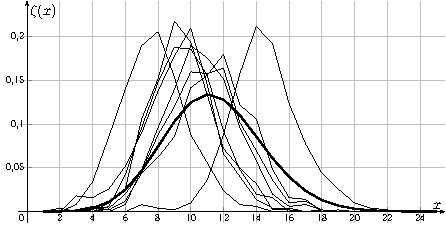
\includegraphics[width=\linewidth]{2019_miet_kai_gav_rdp_fullpart_ba}
  \caption{Распределение длин путей  между узлами (жирная линия "--- полное $\zeta(x)$, тонкие "--- его оценки~$\zeta_i(x)$) в~дереве  Барабаши"--~Альберт} 
\label{rdp_fullpart_ba}
\end{figure}

Целью вычислительного эксперимента является сопоставление полного $\zeta(x)$ и~его оценок~$\zeta_i(x)$, а~также их характеристик,
в~частности, асимметрии и~эксцесса.

Так как  граф $G$ является моделью сетевого уровня сети, использующей стек протоколов TCP/IP,
% Для наилучшего соответствия сетевому уровню сети TCP/IP 
$G$ должен быть связным деревом.
Сложность поиска в~ширину для дерева составляет $O(|G|)$, таким образом, сложность расчёта всех возможных путей составляет $O(|G|^2)$.


Были использованы несколько алгоритмов для генерации связного дерева $G$.
Прежде всего исследована знаменитая модель Барабаши"--~Альберт~\cite{ba} (типичные результаты прогона модели, то есть полное $\zeta(x)$ и~его оценки, показаны на рис.~\ref{rdp_fullpart_ba}).
% На рис.~\ref{rdp_fullpart_ba} показан типичный пример графика $\zeta(x)$ (жирная линия) и~$\zeta_{i}(x)$ (множество тонких линий) РДП для модели Барабаши"--~Альберт.

Полное $\zeta(x)$ для деревьев Барабаши"--~Альберт очень похоже на дискретизацию нормального.
Все они унимодальны.
Большинство оценок $\zeta_i(x)$ рис.~\ref{rdp_fullpart_ba} выглядит более островершинными, чем полное $\zeta(x)$, но менее островершинными, чем распределения, полученные экспериментально (рис.~\ref{zplot_2x1}, а, б).
Рассмотрим характеристики полных распределений и~их оценок подробнее (рис.~\ref{5_moments_ba}).

\begin{figure}[p]
  \centering
  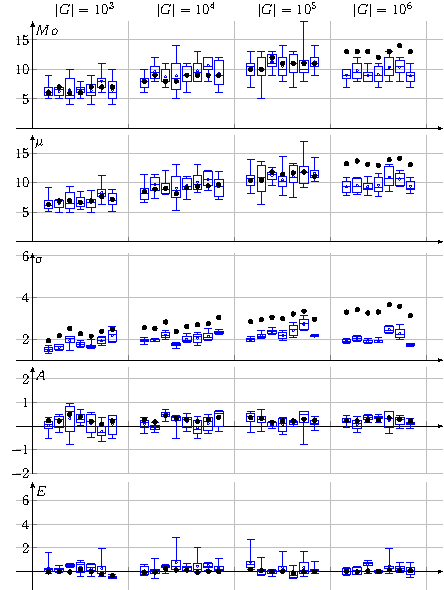
\includegraphics[width=\linewidth]{2019_miet_kai_gav_5_moments_ba}
\caption{Характеристики полного  распределения длин путей в~дереве  Барабаши"--~Альберт (чёрные точки) и~разброс характеристик  его оценок (ящики с~усами)}
\label{5_moments_ba}
\end{figure}

Так как один прогон модели соответствует множеству 
% экспериментальных измерений,  
оценок, а~в~процессе исследования было выполнено множество прогонов, визуализировать характеристику каждой конкретной оценки аналогично рис.~\ref{5x2_experiment_moments} нерационально.
Соответственно, один прогон на рис.~\ref{5_moments_ba} соответствует одной вертикали (по оси абсцисс откладывается номер смоделированного графа; измерения сгруппированы по количеству $|G|$ вершин в~графе).
Для каждого прогона и~каждой характеристики показан разброс значений характеристики $\zeta_i(x)$ в~виде ящика с~усами (аналогично показанному слева на рис.~\ref{5x2_experiment_moments});
кроме того, чёрной точкой на рис.~\ref{5_moments_ba} показано значение характеристики $\zeta(x)$ (для экспериментальных данных его аналог "--- характеристика $\zeta(x)$ глобальной сети "--- недоступна и~поэтому отсутствует на рис.~\ref{5x2_experiment_moments}).

Видно, что асимметрия полных распределений $\zeta(x)$ для деревьев Барабаши"--~Альберт несколько больше нуля, но не достигает полученных в~результате эксперимента значений $3-4.5$.
Асимметрия оценок $\zeta_i(x)$ может быть как больше, так и~(что чаще) ещё меньше асимметрии $\zeta(x)$.
С~ростом количества $|G|$ вершин в~графе  асимметрия как $\zeta(x)$, так и~$\zeta_i(x)$ не растёт.

Эксцесс полных распределений $\zeta(x)$ для деревьев Барабаши"--~Альберт близок к нулю.
Эксцесс оценок $\zeta_i(x)$ может быть как больше (что чаще), так и~меньше эксцесса $\zeta(x)$,
при этом ни одна из этих величин не достигает полученных в~результате эксперимента значений $20-30$.
С~ростом количества $|G|$ вершин в~графе  эксцесс как $\zeta(x)$, так и~$\zeta_i(x)$ не растёт.

Погрешность оценивания асимметрии достигает 100\%, а~эксцесса "--- 1000\% (последнее обусловлено близостью к~нулю эксцесса  $\zeta(x)$).


Таким образом, различие между асимметрией и~эксцессом экспериментально полученных для сетевого уровня глобальной сети данных и~распределениями длин путей в~деревьях Барабаши"--~Альберт обусловлено не случайными отклонениями, не методикой измерения
и~не отличием в~размерах (асимметрия и~эксцесс мало изменяются при росте $|G|$).

Соответственно, различие должно быть обусловлено моделью роста дерева.
В~исследовании были рассмотрены несколько моделей роста.
Наиболее перспективной выглядит предфрактальная модель, описывающая рост сети как рост множества связанных друг с~другом подсетей (рис.~\ref{rdp_fullpart_pfk_32} и~\ref{6_moments_pfk_32}).

\begin{figure}[!h]
  \centering
  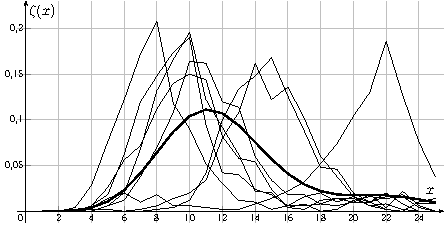
\includegraphics[width=\linewidth]{2019_miet_kai_gav_rdp_fullpart_pfk_32}
  \caption{Распределение длин путей между узлами (жирная линия "--- полное $\zeta(x)$, тонкие "--- его оценки~$\zeta_i(x)$) в~предфрактальном дереве} 
\label{rdp_fullpart_pfk_32}
\end{figure}

\begin{figure}[p]
  \centering
  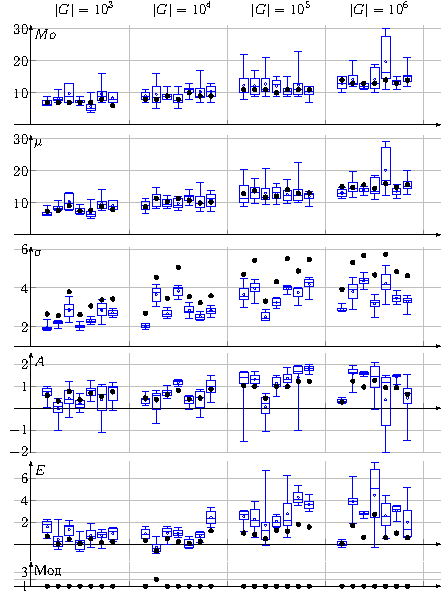
\includegraphics[width=\linewidth]{2019_miet_kai_gav_6_moments_pfk_32}
\caption{Характеристики полного распределения длин путей в~предфрактальном дереве (чёрные точки) и~разброс характеристик его оценок (ящики с~усами)}
\label{6_moments_pfk_32}
\end{figure}%

Вид полного $\zeta(x)$ и~его оценок $\zeta_i(x)$ для одного из прогонов модели представлен на рис.~\ref{rdp_fullpart_pfk_32}.
На рис.~\ref{6_moments_pfk_32} этот прогон "--- первый в~группе $|G|=10^5$.

Так как подсети формируются при росте графа случайным образом,
полные $\zeta(x)$ для предфрактальных деревьев более разнообразны, чем для деревьев Барабаши"--~Альберт.
Некоторые из них не унимодальны.
Соответственно, на рис.~\ref{6_moments_pfk_32}
в~числе прочих характеристик показано и~количество выраженных максимумов $\zeta(x)$.
В~остальном организация рис.~\ref{6_moments_pfk_32} аналогична рис.~\ref{5_moments_ba}.

Распределение $\zeta(x)$ на рис.~\ref{rdp_fullpart_pfk_32} отличается от рис.~\ref{5_moments_ba} наличием толстого правого хвоста.
% ,
% % который, хотя и~не формирует 
% Это "--- наиболее типичная форма $\zeta(x)$ предфрактального дерева.
% Тем не менее, в~зависимости от соотношения размеров подсетей $\zeta(x)$ может иметь
В~целом, в~зависимости от соотношения размеров подсетей 
% % а~также соединений 
$\zeta(x)$ предфрактального дерева может иметь как более или менее толстый правый хвост, аналогичный рис.~\ref{rdp_fullpart_pfk_32}, так и~
один или несколько ярко выраженных побочных максимумов (второй прогон в~группе $|G|=10^5$), либо, наоборот, может иметь тонкий хвост, как для $\zeta(x)$  деревьев Барабаши"--~Альберт (первый прогон в~группе $|G|=10^6$ "--- в~процессе роста сформировалась только одна крупная подсеть).

Соответственно, разброс как характеристик $\zeta(x)$ для разных прогонов, так и~их оценок $\zeta_i(x)$ для одного прогона модели на~рис.~\ref{6_moments_pfk_32} больше, чем на~рис.~\ref{5_moments_ba}.

Асимметрия и~эксцесс $\zeta(x)$ первого прогона в~группе $|G|=10^6$ (с~единственной крупной подсетью) ожидаемо близки к~асимметрии и~эксцессу $\zeta(x)$  деревьев Барабаши"--~Альберт, а~их оценки имеют столь же маленький разброс.

Асимметрия полного $\zeta(x)$ второго прогона в~группе $|G|=10^5$ (с~двумя конкурирующими подсетями, то есть практически одинаковыми максимумами) положительна, 
при этом асимметрии её оценок могут принимать и~отрицательные значения.
Эксцесс полного $\zeta(x)$ и~большинство его оценок отрицательны, так как два близких максимума суммарно массивнее хвостов распределения.

Для всех прочих прогонов асимметрия и~эксцесс положительны, а~их оценки в~подавляющем большинстве завышены.
При этом с~ростом $|G|$ увеличивается и~разброс распределений длин путей от прогонов, и~абсолютная величина асимметрии и~эксцесса.

Погрешность оценивания асимметрии достигает 100\%, а~эксцесса "--- 500\%.


\subsection*{Заключение}

Инструментальные средства, стандартные для большинства дистрибутивов GNU/Linux, а~также GNU Octave, позволяют выборочно оценить распределение длин путей между узлами в~глобальной сети.

Имитационное моделирование позволяет утверждать, что, несмотря на гигантскую погрешность оценивания асимметрии и~эксцесса описываемым методом, полученные экспериментальные данные позволяют уверенно утверждать, что сетевой уровень глобальной сети не описывается моделью Барабаши"--~Альберт, но может быть в~некотором приближении описан разработанной  предфрактальной моделью.

 
\begin{thebibliography}{9}
\bibitem{muchos} {Кононова А. И., Городилов А. В., Шаньгин В. Ф. Особенности передачи
данных в децентрализованных пиринговых сетях // Изв. вузов. Электроника
(ВАК). 2012. No 6(98). С. 95.
}
\bibitem{Sedgewick2002_AlgorithmsinC_Fundamentals} {Седжвик Р. Фундаментальные алгоритмы на С++: Алгоритмы на графах.
СПб: Диа Софт, 2003. 1136 с.
}

\bibitem{ba} {Jeong H., Tombor B., Albert R. et al. The Large-Scale Organization of Metabolic Networks. 2000. \url{https://arxiv.org/pdf/cond-mat/0010278.pdf}
}

\end{thebibliography}

\end{document}
